% !TEX TS-program = lualatex
% !TEX encoding = UTF-8 Unicode
\documentclass [a4paper, 11pt] {article}
\usepackage[a4paper, total={16cm, 26.2cm}]{geometry}
\usepackage[ngerman]{babel}
\usepackage{fontspec}
\usepackage{tabularx}
\usepackage{url}
\usepackage{tikz}  
\usepackage{siunitx}
\sisetup{output-decimal-marker = {,}}
\sisetup{per-mode=fraction}
\pagestyle{empty}

\begin{document}

\begin{center}
{\sf\LARGE Frank macht's}
\par\medskip
{\sf Eine Kalendergeschichte}
\end{center}\par

\noindent Ach Du Heilige Scheiße! Mit einem Schwur auf den Lippen, war Frank hineingetreten. Es war ein klarer kühler Novembertag. Frank sah nach unten auf den Bürgersteig und, um das Wort noch einmal auszusprechen, auf die Scheiße. Seine Nase, sich den Gerüchen der Stadt für gewöhnlich verschließend, nahm Witterung auf und bestätigte: Frank war voll in die Scheiße getreten.

Was tun? Frank beugte sich nach unten. Mit spitzen Fingern zog er den beschmierten Schuh, einen blauen Addidas, aus und balancierte, etwas wackelig, auf einem Bein. Dann richtete er sich wieder auf und warf den Schuh einem vorbeifahrenden Auto hinterher. 

Das Auto jedoch, ein pinkfarbener BMW 323, Baujahr 1983, fuhr weiter. Sein nun nur mit einem Socken bekleideter Fuß drückte aufs Gaspedal, und 150 Pferde beschleunigten den Wagen auf \SI{60}{\km/\hour}. Frank versenkte sich in den kultivierten Sound des Reihensechszylinders, genoss die angenehmen Vibrationen in seinem Körper und fokussierte sich ganz auf seine Mission. 

Eine Schrecksekunde später stieg Frank aufs Bremspedal und brachte den Wagen zum Halt. Vor ihm hatte eine alte Dame ihren Rollator auf die Straße geschoben und schickte sich an, die Fahrbahn zu überqueren. Frank staunte, denn an einem Bein, so glatt und weiß wie Elfenbein, war ihre Hose hochgekrempelt. 

Schritt für Schritt schob sich die Dame nach vorne. Wie eine Raupe stützte sie sich abwechselnd, ihr Elfenbein nachziehend, auf ihren Rollator, um dann wieder den Rollator nach vorne zu schieben. Frank wurde ungeduldig. Er drückte das Gaspedal durch und brachte sein Kraftzentrum, ohne eingelegten Gang, auf 8000 Umdrehungen. Geil. Er hatte schon immer mal einen Achttausender besteigen wollen.

Nur mit Mühe, den Rollator voraus, erklomm Frank den Bordstein zum Mittelstreifen. Ein kleiner Schritt für die Menschheit, ein großer für den einbeinigen alten Herrn. Frank verharrte einen Moment auf dem mit Graß bewachsenen Mittelstreifen und genoss die monumentale Zentralperspektive der einstigen Promenade, den links und rechts vorbeiströmenden Verkehr.

Als eine entfernte Ampel auf Rot schaltete und der Strom der Fahrzeuge pausierte, gab Frank seinem Rollator einen Stoß, so dass dieser zur anderen Straßenseite schleuderte. Frank selbst ließ sich von der Bordsteinkante nach vorne fallen und verlagerte sein Gewicht auf das Elfenbein, an dessen unterem Ende das Zwillingsrad eines Einkaufswagens montiert war. So rollte er, sein linkes Bein anmutig nach hinten streckend, in die Abendsonne, die durch eine Baulücke auf der anderen Straßenseite schien. Wie eine Möwe breitete Frank seine Arme aus.

Auf der anderen Straßenseite empfing ihn seine Tante und hakte ihn unter. Mit Tesakrepp band sie die Schaufensterpuppe am Rollator fest: eine lange Schlaufe um die Hüfte, dann mehrmals um den linken und den rechten Griff gewickelt. Den Rollator wiederum stellte sie neben der Schwitzhütte ab, mit der ein alternatives Unternehmerkollektiv die Baulücke zwischennutzte.

Frank öffnete die Türe zum Vorraum, und gleich umarmten ihn eine wohlige Wärme und der Geruch von Menschen. Ein mit Mini-LEDs dekorierter Tannenbaum verstrahlte ein von einer rotierenden Diskokugel vielfach gebrochenes Licht. Frank legte seine Kleider ab und wartete mit den anderen auf den Einlass in die Sauna. 

Ein Gong gab das Zeichen zum Eintritt. Mit einem Dutzend anderer Schwitzwilliger ging Frank in den Saunaraum und setzte sich auf eine der oberen Bänke. Die Luft war zum Schneiden. Im Zentrum des Raumes, auf einem abgesägten Baumstamm, dampfte eine Glaskugel mit Glühwein, von der Hitze des Saunaofens auf Temperatur gebracht, und würzte den Luft, gleich einem Aufguss, mit Süße und Alkohol. Ein langer Strohhalm, gleich einem Spinnenbein, wurde herumgereicht, durch den die Gäste vom Glühwein trinken konnten. Auch Frank nahm einen Schluck und gab sich ansonsten der Hitze hin, um alle Gedanken und sich selbst aufzulösen.

%Frank wählte jedoch eine der Atemmasken, die Gäste davor bewahrten, Alkohol einzuatmen und transzendent zu werden. Er setzte die Maske auf, die sein Gesichtsfeld einschränkte und ihm auch willkommen war, nicht auf die entblätterten Leiber der anderen Gäste starren zu müssen. Als besonderes Angebot konnte man sich nach dem Saunagang aus dem in der Maske gesammelten Gesichtsschweiß einen isostonischen Cocktail mixen lassen. Frank löste sich in der Hitze auf.

Nach fünfzehn Minuten weckte ihn wieder der Gong. Frank ging zurück in den Vorraum und kleidete sich an. Das Ritual hatte ihn etwas gelehrt: Nie mehr würde er mit dem Schicksal hadern, nicht mit seinem eigenen, und nicht mit dem Schicksal der Menschheit. Mit diesem Schwur ging Frank nach draußen. Auf dem Bürgersteig schichtete sich herabgefallenes Herbstlaub. Ach Du Heilige Scheiße!
\begin{center}
%\vspace{-\baselineskip}
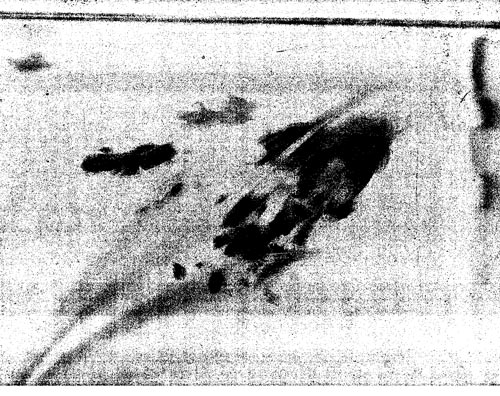
\includegraphics[height=0.7cm]{../jumper}%
\end{center}

\end{document}
